\chapter{Design}

	My first aim, while starting the design part, was to produce a set of interfaces which could possibly support not only my particular game, but a various range of games which could base themselves on the same abstract logic.
	In particular, RTS AR games could be easily derived from the classes I produced for my project.
	Proceeding with the code writing I noticed that my aim was partially infeasible, for example in my try of generalize various type of games (Turn based, Checkpoint based, etc.) and location management, due to Java code rules and limitations in terms of Inheritance and Polymorphism.
	To overcome those limitations I would had to change the way my core interfaces worked, so I preferred to lower a bit the aim and to keep project-independent interfaces only for the really basic concepts.

	\section{Game Rules}
		
		Most of the rules of reference board game has been kept while translating the rules to the app; the most notably difference are the player management and the card system removal.
		
		\subsection{Leaders and Units}
		
			While in the original game we had 2-4 players, now we have 2-5 (and even more) teams, composed by 1 leader and 4-6 units each.
			The leader will represent the player of the original game, while units are the minions he would move; following this idea, the leader will be a strategist which will guide the units, like if he would be a player of an RTS game coordinating his units.
			More specifically, leaders of all the teams will be conduced in a room with a PC ready for every one and from there will be able to see everything that is going on in the board via a web-app: ally units, enemy units, their movements during the game, etc.
			The leader will be able to communicate to minions both in a textual or audio way, guiding them and telling them the enemy moves.
			They'll as well be the managers of the team gold reserve, lending money to units at the start of the turn, which will return into the team reserve at the end of the turn, if not used.
			Also a part of the role management will depend by leaders, as described below.
		
		\subsection{Board and Zones}\label{design:board}
		
			Board concept has been retained unchanged from the original game, but instead of a physical one in cardboard, a virtual one is generated on-the-fly starting from given centre and radius.
			The algorithm currently generate a pseudo-circular board with nine zones displaced in a symmetric way, with a central zone, 4 zones on the inner ring and 4 zones in the outer ring shifted by 45° with respect to the inner one.
			
			\begin{figure}
				\centering
				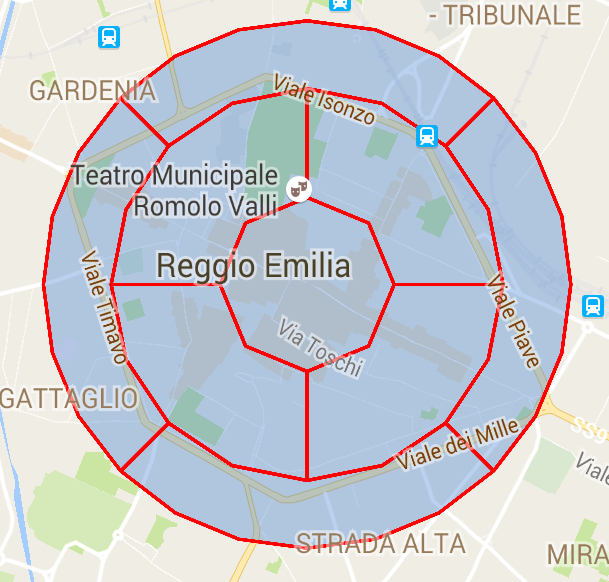
\includegraphics[width=.5\textwidth]{rightboard}
				\caption{Ideal shape of the board and zones}
			\end{figure}
			
			Zones all have the same area, thanks to a R simulation which calculated the right radius to use for different coordinates rings.
			Ideally, moving from a zone centre to another zone centre shall take 5 minutes and turn duration is related to this: the players shall make a choice between moving slightly (one zone or even staying in the same zone) and get plenty of time to perform their actions or move a lot (two or three zones) and running out of time to anything.
			Every zone grants a power-up when teams build on them (higher the building cost, more useful is the power-up) and the zones are randomly distributed on the board (eg. the power-up disposition will be unlikely to be repeated in subsequent games).
			Power-up activate at the begin of every turn.
			
			On a board of 9 zones, power-up are defined as in \autoref{powup:desc}, notice that some of them are referred to the role system, explained in the next subsection.
			
			\begin{table}
				\caption{Power-up description}
				\label{powup:desc}
				\centering
				\begin{tabular}{lccp{0.5\textwidth}}
					\toprule
					Name 			& Number 	& Cost 	& Description \\
					\midrule
					Money 			& 2 		& 4 	& Gain 3 coins \\
					Money 			& 2 		& 7 	& Gain 5 coins \\
					Calm 			& 1 		& 7 	& If the zone with power-up is chaotic, it is no more chaotic. Otherwise, calm a nearby chaotic zone, if more than one is present, it gets randomly chosen between the available ones \\
					Role 			& 2 		& 4 	& Gain one extra cop, assassin and builder role in your role pool \\
					Untouchable 	& 1 		& 9 	& You gain an untouchable bonus role: the player who get this cannot be killed \\
					Multitasking 	& 1 		& 9 	& You gain a multitasking bonus role: the player who get this can use both his actions for this turn \\
					\bottomrule
				\end{tabular}
			\end{table}
		
		\subsection{Roles and Actions}
		
			The card system had to be removed because, while easy to realize and use for single players, it would be too complex, time consuming and random based to use in a team-based game, especially if used through an app for mobile devices.
			But removing the card system come to a price, leaving a hole in the game mechanics behind himself: action assignment.
			To fill this hole, we prepared a new system based on roles, with the main objectives of creating a system which could let enough freedom of act to units, in order to remove the feeling of just being minions controlled by the leaders, and create a balanced game play.
			In this system only three main roles and a filler one, always available, can be used, everyone with it's actions and visibility rule particularities.
			In addition every role, except the filler one, must choose to perform an action between the two provided.
		
			\begin{description}
				\item[cops] can see their team mates and all assassins in the zone.
					\begin{description}
						\item[protect] all allies units within 10 meters to him cannot be killed.
						\item[calm down] following a path of randomly generated coordinates inside the current zone, the zone won't be chaotic any more.
					\end{description}
				\item[assassins] can see their team mates and all builders in the zone.
					\begin{description}
						\item[assassinate] if the zone is chaotic and he manage to stay within 10 meters to an enemy for at least 5 seconds, that enemy won't be able to use his action for the rest of the turn. If the assassinate unit owns money, the assassin rob it.
						\item[tear down] demolish a building, the owner team get refunded with half the price of the building and lose the zone power-up.
					\end{description}
				\item[builders] can see all other units in the zone, but does not know their role.
					\begin{description}
						\item[build] if the zone is not chaotic and the builder manage to stay near a randomly generated point in the zone for 2 min playing a small AR mini-game, a building owned by his team will rise there, provided he has enough money, and grant a power-up.
						\item[spread panic] following a path of randomly generated coordinates inside the current zone, it will become chaotic, if it was not already.
					\end{description}
				\item[collectors] can see only their team mates in the zone and money-grab points, but he knows the number of the other collectors in his same zone.
					\begin{description}
						\item[collect money] every time he reach a money-grab point, he earn one coin. Money-grab points are shared between all team and spawn in random locations on the board at the start of a every new turn.
					\end{description}
			\end{description}
			
			Roles has been defined to counter one other: cops can prevent the assassins to do their job, assassins are mainly equipped to attack builders and tear down what they made and builders hinder cops work by spreading the panic in a zone or trying to get the zone power-up.
			
			Some special roles, called bonus roles or enhancer roles, are earned as a consequence of particular power-ups, can be assigned by the leader to units, extra to the one usually distributed, and expires after one usage.
			Those roles change some in-game rules for the owners:
			\begin{description}
				\item[untouchable] the unit cannot be killed, either by assassins or events;
				\item[multitasking] the unit can perform both the actions of the primary role he chose.
			\end{description} 
			
			Role system is managed by leaders and units together.
			At game start, units own three roles (one per type) and leaders own six roles (two per type).
			During the start of each turn except the first, the leaders can give a role to every unit, taken from their role pool, and units will decide which role and associated actions will use for this turn.
			At the end of each turn every unit that used his action successfully will refund the spent role, which will be added to the leader role pool, ready to be redistributed on the subsequent phase; if the unit get assassinated or do not use the action he chose, the role will still be added to the leader pool, but on the subsequent turn.
			
			This system has been thought in order to give the leaders a way to "set the path" for his units, but still to let the units decide independently if they think that a different action will be more useful in that moment.
		
			% INSERT ROLE SYSTEM IMAGE HERE
			
			When giving out roles, leaders can also assign a mission to every unit which consist of a role, an action and a target (another unit or a zone).
			The unit can decide to accept the mission or to ignore it. If the unit decide to accept it, his role and actions are set automatically to the suggested ones and he'll see additional informations about his target (his positions, how many units are in the particular area, etc.) depending on the mission nature. If he accomplishes the mission, the team gain a small money bonus.
			
		\subsection{Starting zones}
			
			Various ideas had been evaluated to decide how the units should start.
			The main ones where: 
			
			\begin{enumerate}
				\item Following the original game, three fixed zones shall be the starting ones for every team, with the units equally distributed on them;
				\item All units start in the central zone;
				\item Units start from three fixed zones, but divided by team, instead of being equally distributed.
			\end{enumerate}
			
			The first option could be a problem in terms of organization, because every team start already divided and cannot make plans before the game start, thus bounding even more the units to instructions and suggestion given by the leader.
			But on another level, is the option that grant the more equilibrated start in terms of interaction between teams.
			
			The second one could seem funny at a first glance, but it will probably result in havoc and just a few of the units in game to actually succeed in their action for the first and second turn, slowing down the game.
			
			Third option has the exact opposite effect: for the first turns, teams will not interact at all or will do it very little and will only build on the zones near their starting zones or collecting money, thus crippling the game at the very beginning and giving a feeling of boredom. 
			
			Finally, the first option was selected for testing, even if the starting zones now are being randomly chosen instead of being fixed.
			% REVIEW, POWER-UP ARE STILL FIXED
			In fact, the main reason for which they where fixed in the first place, was that also the zones power-up where fixed: now that the power-up disposition is randomly generated, also the starting zone can be randomly chosen.
			
			All starting zones are set as chaotic by default.
		
		\subsection{Objectives}
			
			The objective system, which assigned a different one to every player, has been retained and most of the objectives are inspired to the ones of the board game. Leaders do not know which team has which objective (except his, obviously), but can deduce it from other teams actions and behaviour, since they will be informed of all objective in play, and try to hinder other teams.
			
			The objectives are defined as:
			\begin{description}
				\item[chaos] seven zones are chaotic;
				\item[peaceful] there are no chaotic zones or it's the eighth turn and nobody won;
				\item[omnipresent] there is at least one active unit (which has not been killed in the previous turn) or building on at least eight different zones;
				\item[control] the team controls (has more units+buildings on that zone of every other team) four zones;
				\item[rich] the team money reserve is at least of 50 coins (buildings add up to the money reserve as their's construction cost).
			\end{description}
			
			It's important to remind that objective accomplishment is checked at the very beginning of each turn: the team must keep the victory condition true until the current turn ends.
			
		\subsection{Random events}
			
			The random events effects did not change much from the original game, but of course their occurrence, which was bounded to the card system, had to be updated. Now the event occurrence is related to a certain probability which increase every turn in which no event take place, and reset to a minimum when one of them actually take place.
			
			The events are defined as:
			\begin{description}
				\item[a drake attack the city] extract a zone, all buildings in there are destroyed and all units currently there dies;
				\item[a fire breaks out] extract a zone, buildings in that zone are destroyed and another zone is extracted. If this new zone is nearby the previous one and contains buildings, the fire spreads and they are destroyed as well, then keep extracting a new zone until it stop spreading;
				\item[the fog falls on the city] visibility of each player toward others is blocked, both of team mates and enemies;
				\item[an explosion take place] extract a zone, buildings in that zone are destroyed;
				\item[time to pay taxes] every team must pay 3 coin for every building it owns or destroy it. Payment is done automatically in zone number order;
				\item[suddenly, earthquake] extract two zones, all building in there are destroyed;
				\item[a political disaster] extract a zone, since now the power-up of that zone is disabled for the entire match;
				\item[demons from below] extract five zones, a demon appears on each of those zones, more demons can appear in the same zone. As long as a demon is in it, the zone power-up is disabled, no coins are generated and it's not possible to build. Demons can be killed by assassins via an AR mini-game and have multiple lives.
			\end{description}
			
			Note that when is expressed that buildings are \emph{destroyed}, instead of demolished or tore down, it's meant that the owner team lose the power-up and get no refund; likewise, when is expressed that a unit \emph{dies}, instead of assassinated, it's meant that it lose all the money it was carrying and his role is automatically changed to collector.
			
			
		\subsection{Turns}
		
			The turn mechanics risked to be cut off the final version of the game, because it slowed down the game with respect to a much fluid and free system.
			In the end, we decided to keep it in order to synchronize the various phases (eg. money management, etc.) and avoid problems with the role system: the role refunding would not work in an environment in which all roles did not returned to the leader in the same moment to be distributed again.
			Every turn is divided in two sub-turns: leaders turn, which last 5 minutes and in which all the team management is concentrated, and units turn, which lasts 10-15 minutes and in which the real game take place.
			The basic idea is that leaders will have the 15 minutes of units' turn, while helping them, to define a strategy for next turns; in this way the 5 minutes of their turn are just to formalize and put in place the strategy previously defined.
			
			This is obviously needed also to prevent units from staying still for too much time, which would lead to boredom and ruin the perpetual tension feeling we wanted to grant them.
			
	\section{Variations}
		
		Considering the high team coordination needed to play a game like the one described above, some variations had been prepared to simplify the game and address some mechanics which can be too hard to get for a new player.
		In particular, the fact that leaders do not physically take action in the game could be a problem for various reasons:
		
		\begin{itemize}
			\item a good preparation and knowledge of the game rules is needed to be able to lead the team to victory, which can be hard to achieve in events like the one proposed, because leaders would have only a few hours to prepare: definitely not enough;
			\item while staying in a closed room being the mastermind of your group is could be an interesting idea for someone, there's a possibility that leaders will instead feel isolated and not actively participating to the game;
			\item leader participation would require a web-app development and deployment in order to test also the units part, but this thesis is about the mobile application and the game in itself: this could only slow down the production;
			\item while an app entirely running on smart phone does not require to provide any hardware (everybody have one these days), to use a web app we would need to set up 4-5 computer.
		\end{itemize}
		
		\subsection{Limited leaders}
		
			One possible way to address those problems is reducing leader's duties in the game, removing the web-app necessity and integrating team management in the app.
			In this scenario, leaders plays with their team as they were mere units choosing a role and an action, lose the vision of everything (they only see their team units position) and in general they now look more alike to an on-the-field sergeant or a super-unit than an high level strategist.
			They keep managing the team money reserve and role assignment, but from now on the role pool will be smaller and the system simpler, there won't be missions, for example.
			
			This resolve most of the issues: leaders are now playing with others team members and are generally more involved in the game, no web-app is needed (and thus no computers) and they does not need an in-depth knowledge of the game rules, because they are required only to manage money and a simplified role system.
		
		\subsection{No leaders}
		
			The natural evolution is to remove the leader character at all.
			Here, teams are formed by peer units which together decide where before was leader duty to do so, helped by the app to do so.
			When the team cannot get to a shared decision, the system will follow a default path or choosing randomly between the options, usually resulting a disadvantage to some of the units or to the entire team: this shall convince the team to collaborate in a positive way.
			
			\textbf{The project will implement this variation of the game.}
			
			% FIXED ROLE POOL?
			\subsubsection{Roles}
			\label{nolead:role}
				Role distribution in this scenario change drastically: role pool is fixed (two roles per type, infinite for the filler role) and the role choice is bounded to a timer.
				Every unit must select his preferred role for that turn, if there are left of that kind, and communicate with the team to resolve possible conflicts (eg. three units want to be assassins).
				When the timer stops, every unit get the role he selected and must choose the action. Conflicts are avoided in a first-come, first-served fashion.
				
				Bonus roles are managed more or less in the same way: players can ask to use one of them \emph{in addition} to their preferred role, and conflicts are avoided in the same way as the normal roles.
							
			\subsubsection{Money}
			\label{nolead:money}
				Money distribution is managed similarly: when the turn starts units ask to borrow a certain amount of money from the team reserve, if there is enough money for everyone the money is simply distributed to who asked for them, while if the requested money exceeds the team reserve, units must discuss between them to resolve possible conflicts.
				When the turn ends, money from all units is put back into the team reserve.
				
				This could also be achieved by an on-the-fly request only when the money is needed, but this alternative could bring to even more problems: the rule that allowed assassin to rob his victim partially break apart in this way, because only the collectors (or another assassin which had previously killed a collector) will have money with them, and the loan will probably need a confirmation vote from all others units, wasting a lot of time.
		